
%% The first command in your LaTeX source must be the \documentclass command.
\documentclass[manuscript,screen,review]{acmart}
\usepackage{colortbl}
\usepackage{graphicx}
\usepackage{subcaption}
%%
%% \BibTeX command to typeset BibTeX logo in the docs
\AtBeginDocument{%
  \providecommand\BibTeX{{%
    \normalfont B\kern-0.5em{\scshape i\kern-0.25em b}\kern-0.8em\TeX}}}


%% These commands are for a PROCEEDINGS abstract or paper.
\acmConference[CS 235]{Data Mining Techniques}{Fall 2023}{UCR}
%\acmPrice{15.00}
%\acmISBN{978-1-4503-XXXX-X/18/06}


%%
%% Submission ID.
%% Use this when submitting an article to a sponsored event. You'll
%% receive a unique submission ID from the organizers
%% of the event, and this ID should be used as the parameter to this command.
%%\acmSubmissionID{123-A56-BU3}



%%
%% end of the preamble, start of the body of the document source.
\begin{document}

%%
%% The "title" command has an optional parameter,
%% allowing the author to define a "short title" to be used in page headers.
\title{CS235 Fall'23 Project Implementation Correctness Report: Use Deep Learning to Predict Car Sales Price}

%%
%% The "author" command and its associated commands are used to define
%% the authors and their affiliations.
%% Of note is the shared affiliation of the first two authors, and the
%% "authornote" and "authornotemark" commands
%% used to denote shared contribution to the research.
\author{Liam Hsieh (NetID:lhsie013)}
\affiliation{%
 % \state{862395843 (lhsie013)}
}
\email{lhsie013@ucr.edu}

\renewcommand{\shortauthors}{Liam Y. Hsieh}

%%
%% By default, the full list of authors will be used in the page
%% headers. Often, this list is too long, and will overlap
%% other information printed in the page headers. This command allows
%% the author to define a more concise list
%% of authors' names for this purpose.

%%
%% The abstract is a short summary of the work to be presented in the
%% article.
%%
%% The code below is generated by the tool at http://dl.acm.org/ccs.cfm.
%% Please copy and paste the code instead of the example below.
%%

%%
%% Keywords. The author(s) should pick words that accurately describe
%% the work being presented. Separate the keywords with commas.
\keywords{Car sales price prediction, Neural Networks, Mean Absolute Error (MAE)}

%%
%% This command processes the author and affiliation and title
%% information and builds the first part of the formatted document.
\maketitle


\section{Deep Neural Networks}

\subsection{Cross Validation}

This implemented method is multi-layer Neural Network and network models with different layers and setting are evaluated. 

\begin{table}[h]
    \begin{tabular}{|l|l|l|l|}
    \hline
    \textbf{model} & \textbf{layers} & \textbf{neurons} & \textbf{activation} \\ \hline
    1              & 2                                    & 5-5-15-1         & linear              \\ \hline
    2              & 2                                    & 5-5-15-1         & relu                \\ \hline
    3              & 3                                    & 5-5-10-5-1       & linear              \\ \hline
    4              & 3                                    & 5-5-10-5-1       & relu                \\ \hline
    5              & 4                                    & 5-5-15-15-5-1    & linear              \\ \hline
    6              & 4                                    & 5-5-15-15-5-1    & relu                \\ \hline
    7              & 5                                    & 5-5-15-20-15-5-1 & linear              \\ \hline
    8              & 5                                    & 5-5-15-20-15-5-1 & relu                \\ \hline
\end{tabular}
\caption{All prediction models candidates}
\label{tab:model_options}
\end{table}

Table \ref{tab:model_options} provides an overview of candidate prediction models with different architectures.
\begin{itemize}
\item Layers: indicates the number of hidden layers in each model.
\item Neurons: specifies the number of neurons for each layer, following the format that denotes the configuration of hidden layers.
\item Activation:  indicates the activation function used in each model, which can be either Linear or ReLU.
\item The input and output dimensions are consistent across all models, with the input representing features and the output being a single response.
\end{itemize}

We use mean absolute error (MAE) for the cross validation that the absolute value of the error between the predicted values and the actual values is averaged over all testing data set as the performance measure. The number of replications for each ANN is 10.
To assess the impact of adding more hidden layers to the Artificial Neural Network (ANN) architecture, we conducted an analysis of variance (ANOVA) test followed by Tukey's Honest Significant Difference (HSD) test. The primary objective was to determine whether there were statistically significant differences in the performance metrics as we varied the number of hidden layers. Basically, the ANOVA test was employed to evaluate the overall differences in mean performance across different configurations of hidden layers. MAE was used to quantify the effectiveness of each ANN configuration. To further investigate specific differences between pairs of hidden layer configurations identified by the ANOVA test, we applied Tukey's HSD test. This post hoc test allows for a rigorous pairwise comparison while accounting for the multiple comparisons problem.

\subsection{Experimental results}



The results of ANOVA is that we got 0.0319 as p-value, and the result of Tukey HSD is as follows:  
        
\begin{table}[h]
\begin{tabular}{|l|l|l|l|l|l|l|}
\hline
\textbf{group1} & \textbf{group2} & \textbf{meandiff} & \textbf{p-adj}& \textbf{lower}& \textbf{upper}& \textbf{reject} \\ \hline            
2 layers-linear &  2 layers-relu & -0.0099 & 0.97 & -0.051 & 0.0312 & False \\ \hline
2 layers-linear &3 layers-linear & -0.0085 & 0.9869 & -0.0496 & 0.0326&  False \\ \hline
2 layers-linear &  3 layers-relu &  -0.009 &0.9819 & -0.0501 & 0.0321 & False \\ \hline
2 layers-linear &4 layers-linear &  -0.01 &0.9676 &-0.0511 & 0.031 & False \\ \hline
2 layers-linear &  4 layers-relu &  -0.0152 & 0.809& -0.0562 & 0.0259 & False \\ \hline
2 layers-linear &5 layers-linear & -0.0147 &0.8267 &-0.0558 & 0.0263 & False \\ \hline
2 layers-linear &  5 layers-relu & -0.0156 &0.7881 &-0.0567 & 0.0255 & False \\ \hline
  2 layers-relu &3 layers-linear &  0.0014 &   1.0 &-0.0397 & 0.0425 & False \\ \hline
  2 layers-relu &  3 layers-relu &  0.0009 &   1.0 &-0.0402 & 0.042 & False \\ \hline
  2 layers-relu &4 layers-linear & -0.0002 &   1.0 &-0.0412 &0.0409 & False \\ \hline
  2 layers-relu &  4 layers-relu & -0.0053 &0.9992 &-0.0464 &0.0358 & False \\ \hline
  2 layers-relu &5 layers-linear & -0.0049 &0.9995 &-0.0459 &0.0362 & False \\ \hline
  2 layers-relu &  5 layers-relu & -0.0057 &0.9987 &-0.0468 &0.0354 & False \\ \hline
3 layers-linear &  3 layers-relu & -0.0005 &   1.0 &-0.0416 &0.0406 & False \\ \hline
3 layers-linear &4 layers-linear & -0.0016 &   1.0 &-0.0427 &0.0395 & False \\ \hline
3 layers-linear &  4 layers-relu & -0.0067 &0.9966 &-0.0478 &0.0344 & False \\ \hline
3 layers-linear &5 layers-linear & -0.0063 &0.9977 &-0.0474 &0.0348 & False \\ \hline
3 layers-linear &  5 layers-relu & -0.0072 &0.9949 &-0.0482 &0.0339 & False \\ \hline
  3 layers-relu &4 layers-linear & -0.0011 &   1.0 &-0.0422 &  0.04 & False \\ \hline
  3 layers-relu &  4 layers-relu & -0.0062 &0.9979 &-0.0473 &0.0349 & False \\ \hline
  3 layers-relu &5 layers-linear & -0.0058 &0.9986 &-0.0469 &0.0353 & False \\ \hline
  3 layers-relu &  5 layers-relu & -0.0066 &0.9967 &-0.0477 &0.0344 & False \\ \hline
4 layers-linear &  4 layers-relu & -0.0051 &0.9994 &-0.0462 & 0.036 & False \\ \hline
4 layers-linear &5 layers-linear & -0.0047 &0.9996 &-0.0458 &0.0364 & False \\ \hline
4 layers-linear &  5 layers-relu & -0.0056 &0.9989 &-0.0467 &0.0355 & False \\ \hline
  4 layers-relu &5 layers-linear &  0.0004 &   1.0 &-0.0407 &0.0415 & False \\ \hline
  4 layers-relu &  5 layers-relu & -0.0005 &   1.0 &-0.0416 &0.0406 & False \\ \hline
5 layers-linear &  5 layers-relu & -0.0009 &   1.0 & -0.042 &0.0402 & False \\ \hline
\end{tabular}
\caption{Multiple Comparison of Means - Tukey HSD, FWER=0.05}
\label{tab:Tukey_HSD}
\end{table}

In this case, the p-value is less than the conventional significance level of 0.05, suggesting that there is some evidence of a difference in means among the groups.
However, based on the Tukey HSD results, no pairs of groups show a significant difference in means. All the "reject" values are marked as "False." Therefore, despite the statistically significant ANOVA p-value, the post-hoc Tukey HSD test suggests that the observed differences in means may not be specifically attributed to differences between individual pairs of groups.

\begin{table}[h]
    \begin{tabular}{|l|*{2}{c|}}
    \hline
    &   \textbf{mean} &   \textbf{std. dev}\\ \hline
\textbf{2 layers-linear} & 0.010360 & 0.007321 \\ \hline
\textbf{2 layers-relu} & 0.039120 & 0.022072 \\ \hline
\cellcolor{red} \textbf{3 layers-linear} & 0.007703 & 0.004066 \\ \hline
\textbf{3 layers-relu} & 0.021993 & 0.015098 \\ \hline
\textbf{4 layers-linear} & 0.011014 & 0.004181 \\ \hline
\textbf{4 layers-relu} & 0.021542 & 0.015800 \\ \hline
\textbf{5 layers-linear} & 0.012623 & 0.004956 \\ \hline
\textbf{5 layers-relu} & 0.018909 & 0.013284 \\ \hline       
\end{tabular}
\caption{Mean and Std. deviation of MAE}
\label{tab:mean_std}
\end{table}


Therefore, we summarize the results in Table \ref{tab:mean_std} and also illustrate the results in the Fig. \ref{fig:boxplot}. Although none of them significantly outperforms the others, we finally select 3-layers-linear as our prediction model because it not only has the lowest average MAE (see Fig. \ref{fig:layers}) but also has smallest standard deviation of MAE.

\begin{figure}
    \begin{subfigure}{0.5\textwidth}
        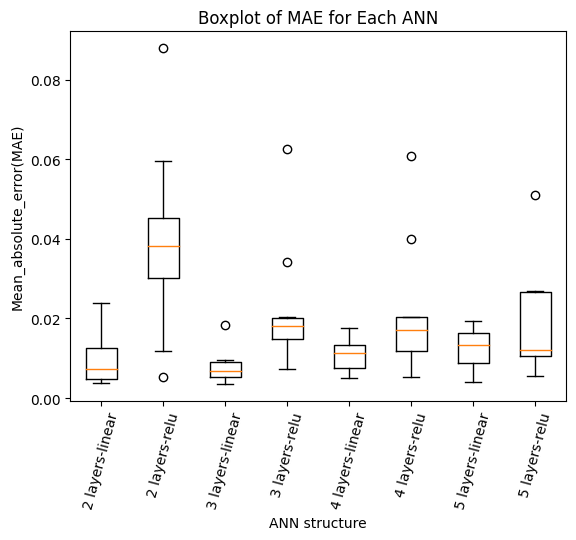
\includegraphics[width=\linewidth]{boxplot.png}
        \caption{Boxplot of different ANN models}
        \label{fig:boxplot}
    \end{subfigure}
    \begin{subfigure}{0.5\textwidth}
        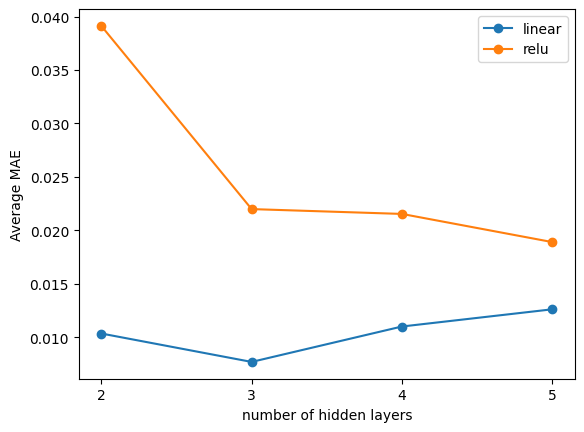
\includegraphics[width=\linewidth]{layers.png}
        \caption{Mean MAE of ANN Models with Varying Number of Hidden Layers}
        \label{fig:layers}
    \end{subfigure}
    \caption{Comparison of ANN models.}
    \label{fig:comparison}
\end{figure}


% \begin{figure}
%     \centering
%     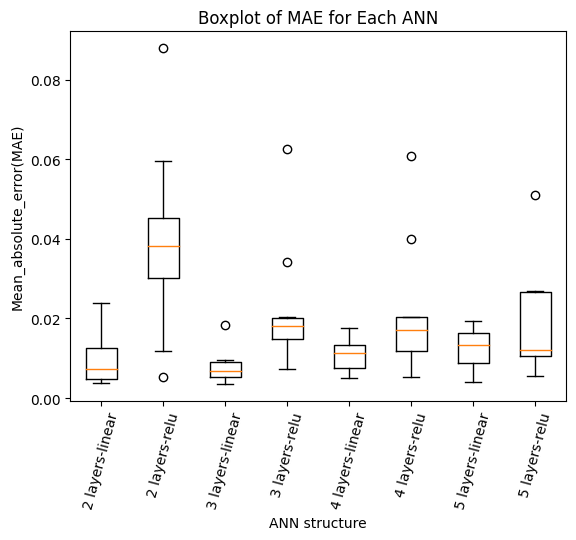
\includegraphics[width=0.5\linewidth]{boxplot.png}
%     \caption{Boxplot of different ANN models}
%     \label{fig:boxplot}
%   \end{figure}

%   \begin{figure}
%     \centering
%     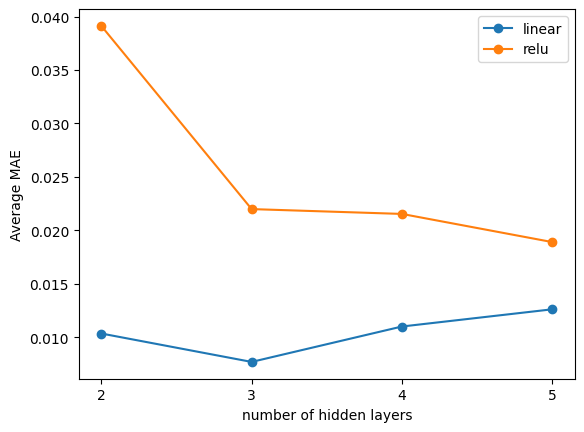
\includegraphics[width=0.5\linewidth]{layers.png}
%     \caption{Mean MAE of ANN Models with Varying Number of Hidden Layers}
%     \label{fig:layers}
%   \end{figure}

\end{document}
\endinput
%%
%% End of file `sample-manuscript.tex'.
